
\lfoot{William Matthews}

\section{Introduction}
\subsection{Project Aims}

In this project a design draft of an ammonia-based Energy Storage System (ESS) is presented.
The plant and wind farm have to power the island of Maui on its own, with no support from other generation units.


\subsection{What is an ESS?}

An Energy Storage System is a means to capturing excess energy in an electrical transmission grid to be used later.
ESSs are seeing an increase in their potential use as many renewables only offer power intermittently, and we see an upwards trend in amount of renewables used \cite{intro:growth}.

%todo explain what it is

\subsection{Location, and why implement an ESS?}
In the scenario given, the plant has to power a location with nothing more than an ESS and a wind farm.
The location chosen (after considering various options through a multi-criteria analysis) was the island of Maui, Hawaii.
The primary considerations leading to the choice of this location were:
\begin{description}
        \item[Fuel Imports]{Hawaii is primarily powered by oil \cite{intro:oilimport} which has to be imported by a fuel tanker. Importing oil adds to the carbon footprint of the generation, as well as the cost of the power made. Eliminating the need to import a fuel via tanker should remove some of the cost associated with generation.}
        \item[High Energy Price]{Hawaii has the highest electrical prices in the USA, at \$0.3114 per kWh (residential January 2018)\cite{intro:price}. The Next highest state is Rhode Island at \$0.2224 per kWh (residential January 2018)\cite{intro:price}. Average US electrical prices across the residential sector is \$0.1223 per kWh (January 2018)\cite{intro:price}. As Hawaii has almost triple the prices across the rest of the US, this seems like a good opportunity for us to penetrate the market with a more cost-effective solution, that the consumers will back.
Hawaii's population is high and it continues to grow year-on-year, meaning extra capacity will have to be built in to satisfy consumer's demands for the future. Of course, as technology and time progresses, the population grows more power-hungry.}
        \item[Clean Energy Initiative]{On January 28, 2008, the State of Hawaii and the USDE (US Department of Energy) signed a `memorandum of understanding' which had the goal to use renewable resources such as wind, sun, ocean, geothermal and bio-energy to supply 70\% or more of Hawaii's energy needs by 2030 to reduce the State's dependence on imported oil.}
        \item[Geography]{Windspeeds in the State of Hawaii are high making this an ideal location for wind power \cite{intro:windspeed}. To supplement this, the U.S. Department of Energy identified Hawaii to have the potential to install 3,000 MW of wind power, capable of generating 12,000 million kWh per year \cite{intro:energy}.
Considering that the entire State used only 9,962 million kWh in 2011, this project seems feasible with efficient processes.}
\end{description}


\subsection{Plant Structure}

The plant structure is setup as in Figure \ref{fig:plantglobaldiagram} and sub-divided into sections for detailed exploration.
This report shows a suggestion as to how the objective of supplying power to Maui can be achieved. 

\begin{figure}[hb]
        \centering
        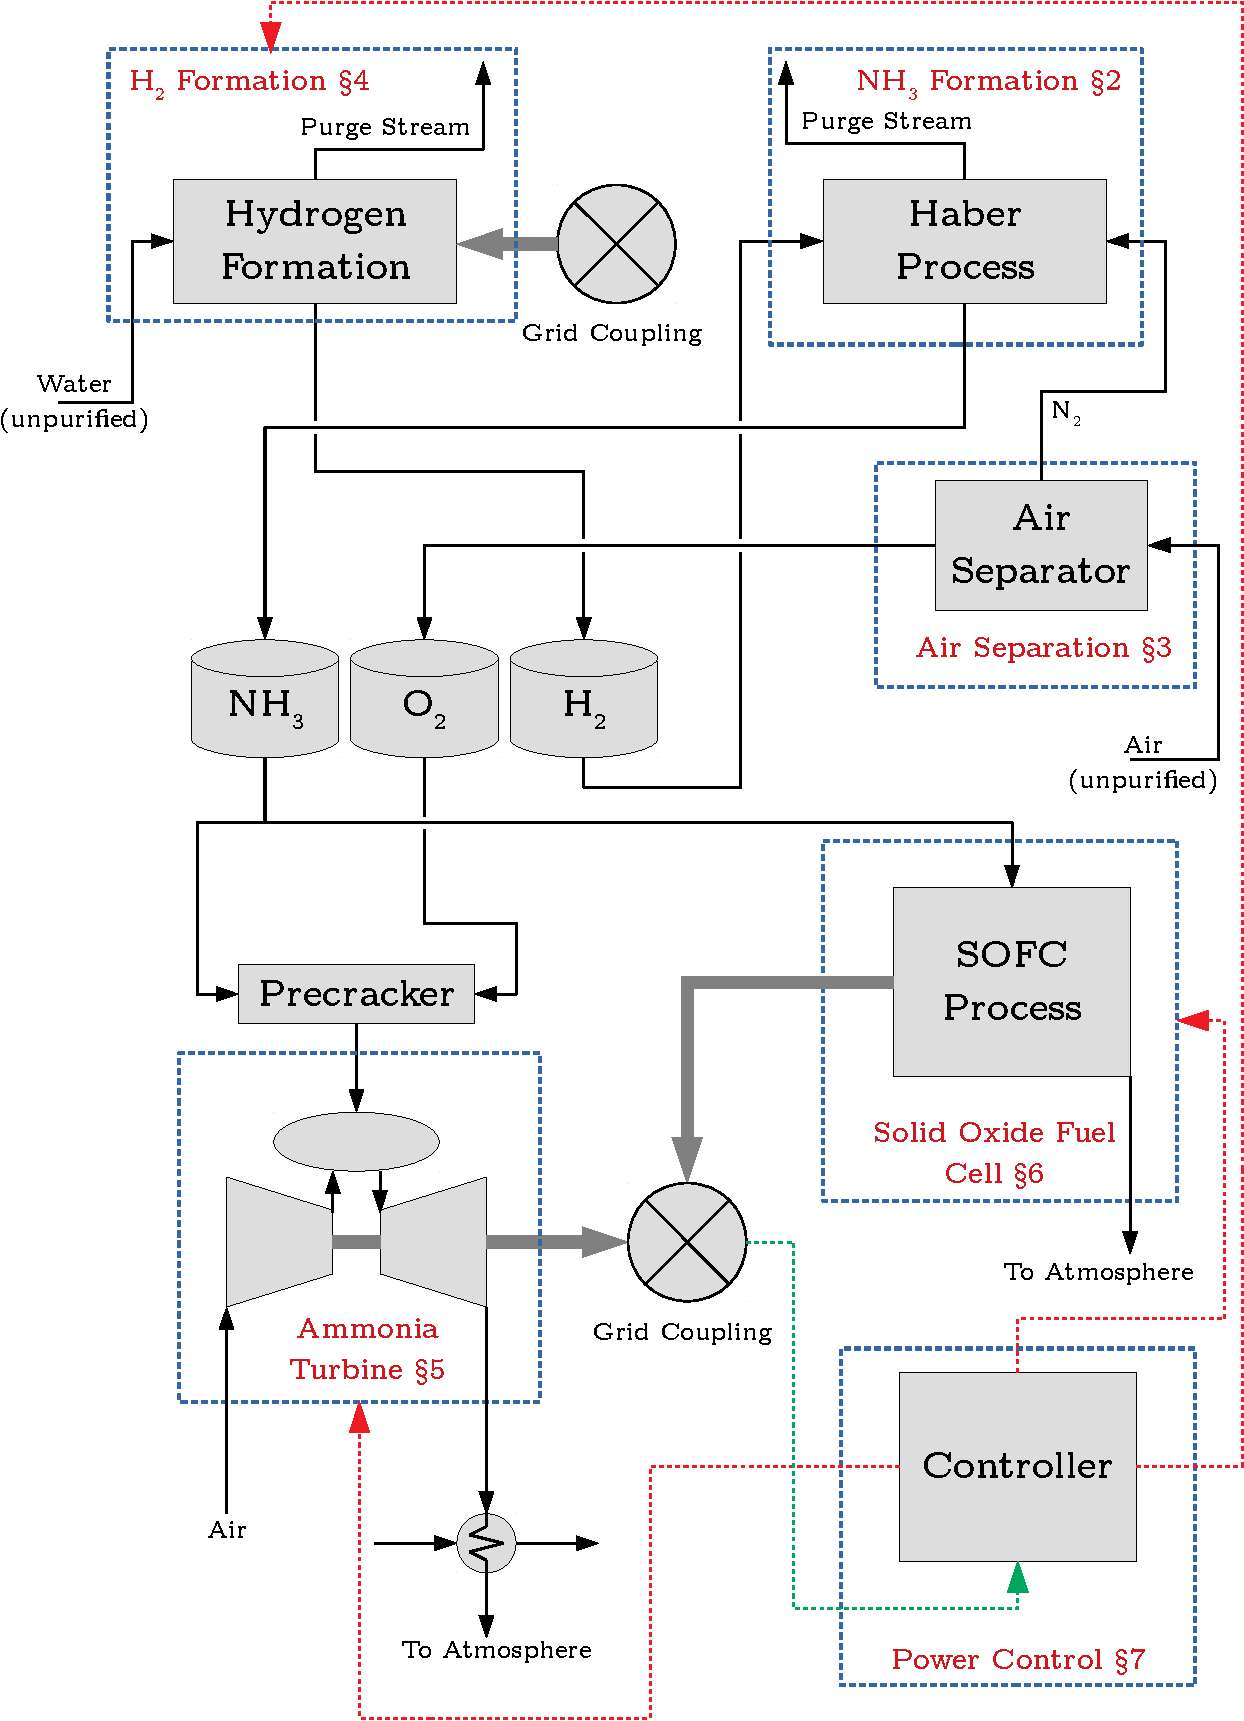
\includegraphics[scale=0.7]{plantdiagram.pdf}
        \caption{Diagram Showing Component Interconnections}
        \label{fig:plantglobaldiagram}
\end{figure}

\begin{thebibliography}{5}
\bibitem{intro:growth}
        Energy Management for Smart Grid, Cities and Buildings: Opportunities for battery electricity storage solutions
        \textbf{YOLE Dev\'eloppement}
        \url{https://www.i-micronews.com/power-electronics-report/product/energy-management-for-smart-grid-cities-and-buildings-opportunities-for-battery-electricity-storage-solutions.html}
        Last Accessed 6 April 2018

\bibitem{intro:oilimport}
        Power Facts
        \textbf{Hawaiian Electric}
        \url{https://www.hawaiianelectric.com/Documents/about_us/company_facts/power_facts.pdf}
        Last Accessed 6 April 2018

\bibitem{intro:price}
        Electric Power Monthly
        \textbf{EIA}
        \url{https://www.eia.gov/electricity/monthly/epm_table_grapher.php?t=epmt_5_6_a}
        Last Accessed 6 April 2018

\bibitem{intro:windspeed}
        NOAA Integrated Surface Database
        \url{https://www.ncdc.noaa.gov/data-access/quick-links#dsi-3505}
        \emph{Data obtained was processed in MATLAB, from ground station Honolulu International Airport}

\bibitem{intro:energy}
        Wind Powering America: Installed U.S. Wind Capacity and Wind Project Locations
        \textbf{Wind Powering America}
        \url{http://www.windpoweringamerica.gov/wind_installed_capacity.asp}
        Last Accessed 10 October 2017
\end{thebibliography}